\documentclass[t]{beamer}
\mode<presentation>{\usefonttheme{serif}}
\beamertemplatenavigationsymbolsempty
\usetheme{metropolis}

\usepackage[utf8]{inputenc}
\usepackage{bbm}
\usepackage{amssymb}
\usepackage{amsmath}
\usepackage[bbgreekl]{mathbbol}
\usepackage[absolute,overlay]{textpos}
\usepackage{graphicx}
\usepackage{tikz}
\usepackage{courier}
\usepackage{ragged2e}
\usepackage{csquotes}

\title{
	{{\Large \textbf{Encontros Matemáticos}} {\small 	apresenta}}\\
\vspace{30pt}
{\huge Computação Quântica}
}
\institute{IM-UFRJ}
\date{19 de novembro de 2019}

\author{Pedro Maciel Xavier \\ \texttt{pedromxavier@poli.ufrj.br}}

\newcommand{\ii}{
	\rm{i}
}


\newcommand{\titulo}[1]{%
	\textbf{\Large #1\\}
}

\newcommand{\teorema}[1]{%
	\textbf{Teorema. (\emph{#1})\\}
}

\newcommand{\prova}{%
	\textbf{Prova.\\}
}

\newcommand{\cqd}{\blacksquare}

\newcommand{\postulado}[1]{%
	\textbf{Postulado. (\emph{#1})\\}
}

\newcommand{\definicao}[1]{%
	\textbf{Definição. (\emph{#1})\\}
}

\newcommand{\vetor}[2]{\ensuremath{
\left[\begin{matrix}
#1 \\
#2
\end{matrix}\right]
}
}

\newcommand{\vetorx}[4]{\ensuremath{
\left[\begin{matrix}
#1 \\
#2 \\
#3 \\
#4
\end{matrix}\right]
}
}

\newcommand{\matriz}[4]{\ensuremath{
\left[\begin{matrix}
#1 & #2 \\
#3 & #4 
\end{matrix}\right]
}
}

\newcommand{\ket}[1]{\ensuremath{\left|#1\right\rangle}}
\newcommand{\bra}[1]{\ensuremath{\left\langle#1\right|}}

\newcommand{\braket}[2]{\ensuremath{\left\langle#1|#2\right\rangle}}

\newcommand{\ketbra}[2]{\ensuremath{\left|#1\right\rangle\left\langle#2\right|}}

\newcommand{\comich}[1]{
	\bgroup
	\setbeamercolor{background canvas}{bg=white}
	\begin{frame}[plain]{}
		\begin{center}
			\begin{figure}
				\includegraphics[height=\textheight]{#1}
			\end{figure}
		\end{center}
	\end{frame}
	\egroup
}

\newcommand{\comic}[1]{\comich{#1}}

\newcommand{\comicw}[1]{
	\bgroup
	\setbeamercolor{background canvas}{bg=white}
	\begin{frame}[plain, c]{}
	\begin{center}
		\begin{figure}
			\includegraphics[width=\textwidth]{#1}
		\end{figure}
	\end{center}
\end{frame}
\egroup
}

\newcommand{\frase}[1]{	
	\begin{center}
		\begin{block}
			~ ''{\small #1}''
		\end{block}
	\end{center}
}

\newcommand{\frasepor}[2]{
	\begin{center}
		\begin{quote}
			#1
		\end{quote}
		\hfill {\small #2}
	\end{center}
}

\newcommand{\comicfinal}[1]{
	\bgroup
	\usebackgroundtemplate{\includegraphics[width=\paperwidth]{#1}}
	\begin{frame}[plain]{}

	\end{frame}
	\egroup
}

\newcommand{\person}[6]{%
% image, name, comment,
% size, dx, dy
\begin{textblock*}{#4}(#5, #6)
	\includegraphics[height=#4]{#1}\\
	#2\\
	{\small #3}
\end{textblock*}
}

\newcommand{\imgw}[2]{%
\begin{center}
	\begin{figure}
	\includegraphics[width=#2]{#1}\\
	\end{figure}
\end{center}
}

\newcommand{\imgh}[2]{%
\begin{center}
	\begin{figure}
		\includegraphics[height=#2]{#1}\\
	\end{figure}
\end{center}
}

\newcommand{\ps}{
	\phantom{-}
}

\newcommand{\HH}{\ensuremath{
	\frac{1}{\sqrt{2}}\matriz{1}{\ps 1}{1}{-1}
}}

\newcommand{\XX}{\ensuremath{
	\matriz{0}{\ps 1}{1}{\ps 0}
}}

\newcommand{\YY}{\ensuremath{
	\matriz{0}{-\ii}{\ii}{\ps 0}
}}

\newcommand{\ZZ}{\ensuremath{
	\matriz{1}{\ps 0}{0}{-1}
}}


%% =====================================================
%% =====================================================
%% =====================================================
%% =====================================================

%% =====================================================
%% =====================================================
%% =====================================================
%% =====================================================

%% =====================================================
%% =====================================================
%% =====================================================
%% =====================================================

\begin{document}

	\begin{frame}
		\titlepage
		\begin{textblock*}{7cm}(8cm, -1.5cm)
			
\includegraphics[width=7cm]{im.pdf}
		\end{textblock*}
	\end{frame}
	
	\begin{frame}{Parte I}
  		\tableofcontents[sections={1}]
    \end{frame}

    \begin{frame}{Parte II}
    \begin{columns}[t]
        \begin{column}{.5\textwidth}
            \tableofcontents[sections={2}]
        \end{column}
        \begin{column}{.5\textwidth}
            \tableofcontents[sections={3-4}]
        \end{column}
    \end{columns}
	\end{frame}

    \begin{frame}{Parte III}
  		\tableofcontents[sections={5-}]
	\end{frame}
	
	

	\section{Computação Digital}
	
	\subsection{O Bit}
	
	\comich{bits0.pdf}
	\comich{bits1.pdf}
	\comich{bits2.pdf}
	\comich{bits3.pdf}
	\comich{bits4.pdf}
	\comicfinal{blue-screen.pdf}
	
	\begin{frame}{\subsecname}
	
	Sobre os \textit{bits}:
		\begin{itemize}
			\item Eles moram em $\mathbb{Z}_2$
			\item Realizamos operações \textit{Booleanas} com eles: $\neg$, $\wedge$, $\vee$, $\oplus$.
			\item Formam vetores em $\mathbb{Z}_2^n$, onde cada $\vec{a} = (a_1, a_2, \dots, a_n) \in \mathbb{Z}_2^n$ representa um valor entre $00...0 = 0$ e $11...1 = 2^n-1$.
			
		\end{itemize}
	\end{frame}
	
	\subsection{Álgebra Booleana}
	
	
	\begin{frame}{\subsecname}
	\definicao{Álgebra Booleana}
	É uma estrutura algébrica $(\Omega, \vee, \wedge, \neg, 0, 1)$, com $0,1 \in \Omega$, que satisfazem os Axiomas:
	
	\footnotesize
		\begin{align*}
			a \vee (b \vee c) = (a \vee b) \vee c && a \wedge (b \wedge c) = (a \wedge b) \wedge c && \text{associatividade}\\
			a \vee b = a \vee a && a \wedge b = b \wedge a && \text{comutatividade}\\
			a \vee 0 = a && a \wedge 1 = a && \text{identidade}\\
			a \vee \neg a = 1 && a \wedge \neg a = 0 && \text{complemento}\\
			a \vee (b \wedge c) = (a \vee b) \wedge (a \vee c) && a \wedge (b \vee c) = (a \wedge b) \vee (a \wedge c) && \text{distributividade}\\
			a \vee (a \wedge b) = a && a \wedge (a \vee b) = a && \text{absorção}
		\end{align*}
	\normalsize
	\end{frame}
	
	\begin{frame}{\subsecname}
		\person{boole.jpg}{George Boole}{1815 - 1864}{4cm}{2cm}{2cm}
		\person{de-morgan.jpg}{Augustus De Morgan}{1806 - 1871}{4cm}{8cm}{2cm}

	\end{frame}

	\subsection{Complexidade e Computabilidade}	
	
	\begin{frame}[label=turing]{\subsecname}
	\titulo{A Tese de Church-Turing}
	
	%% Em 1936, como resposta ao \textit{Entscheidungsproblem} de David Hilbert, Church e Turing publicam resultados independentes mostrando que não existe um algoritmo para determinar se um enunciado da lógica de primeira ordem pode ser provado. Em seu artigo, Turing introduz a \textbf{Máquina de Turing}\\
	
	\frasepor{Toda função que seria naturalmente computável pode ser computada por uma Máquina de Turing}{Alan Turing}
	\end{frame}
	
	\begin{frame}{\subsecname}
	\definicao{Máquina de Turing}
	É um computador abstrato definido por $(Q, q_0, \Gamma, \square, \Sigma, \Omega, \delta)$, que possui uma fita e um cabeçote de leitura
	
	\begin{itemize}
		\item[$Q$:] Um conjunto não-vazio de estados.
		\item[$q_0$:] Estado inicial ($q_0 \in Q$)
		\item[$\Gamma$:] Alfabeto da fita.
		\item[$\square$:] Símbolo vazio.
		\item[$\Sigma$:] Alfabeto de entrada da máquina. ($\Sigma \subseteq \Gamma \slash \{\square\})$ 
		\item[$\Omega$:] Conjunto dos códigos de parada.
		\item[$\delta$:] Função de Transição, $\delta : Q \slash \Omega \times \Gamma \to Q \times \Gamma \times \{\uparrow, \downarrow\}$
	\end{itemize}
	\end{frame}
	
	\begin{frame}{\subsecname}
		\person{church.jpg}{Alonzo Church}{1903 - 1955}{4cm}{2cm}{3cm}
		\person{turing.jpg}{Alan Turing}{1912 - 1954}{4cm}{8cm}{3cm}
	\end{frame}
	
	\againframe{turing}
	
	\begin{frame}{\subsecname}
		\definicao{Complexidade Assintótica}
		Seja $f : X \subseteq \mathbb{R}_+ \to \mathbb{C}$ e $g : X \subseteq \mathbb{R}_+ \to \mathbb{R}_+$ dizemos que
		$$f(x) = O(g(x)) \iff \exists M, x_0 |f(x)| \le M g(x), \forall x > x_0$$
	\end{frame}
	
	\begin{frame}{\subsecname}
	
	\end{frame}


	\comich{first-transistor.pdf}
	
	\subsection{Transistor}	
	
	\begin{frame}{\subsecname}
	
	\end{frame}
	
	\subsection{Portas Lógicas}	
	
	\begin{frame}{\subsecname}
		
		\begin{figure}
			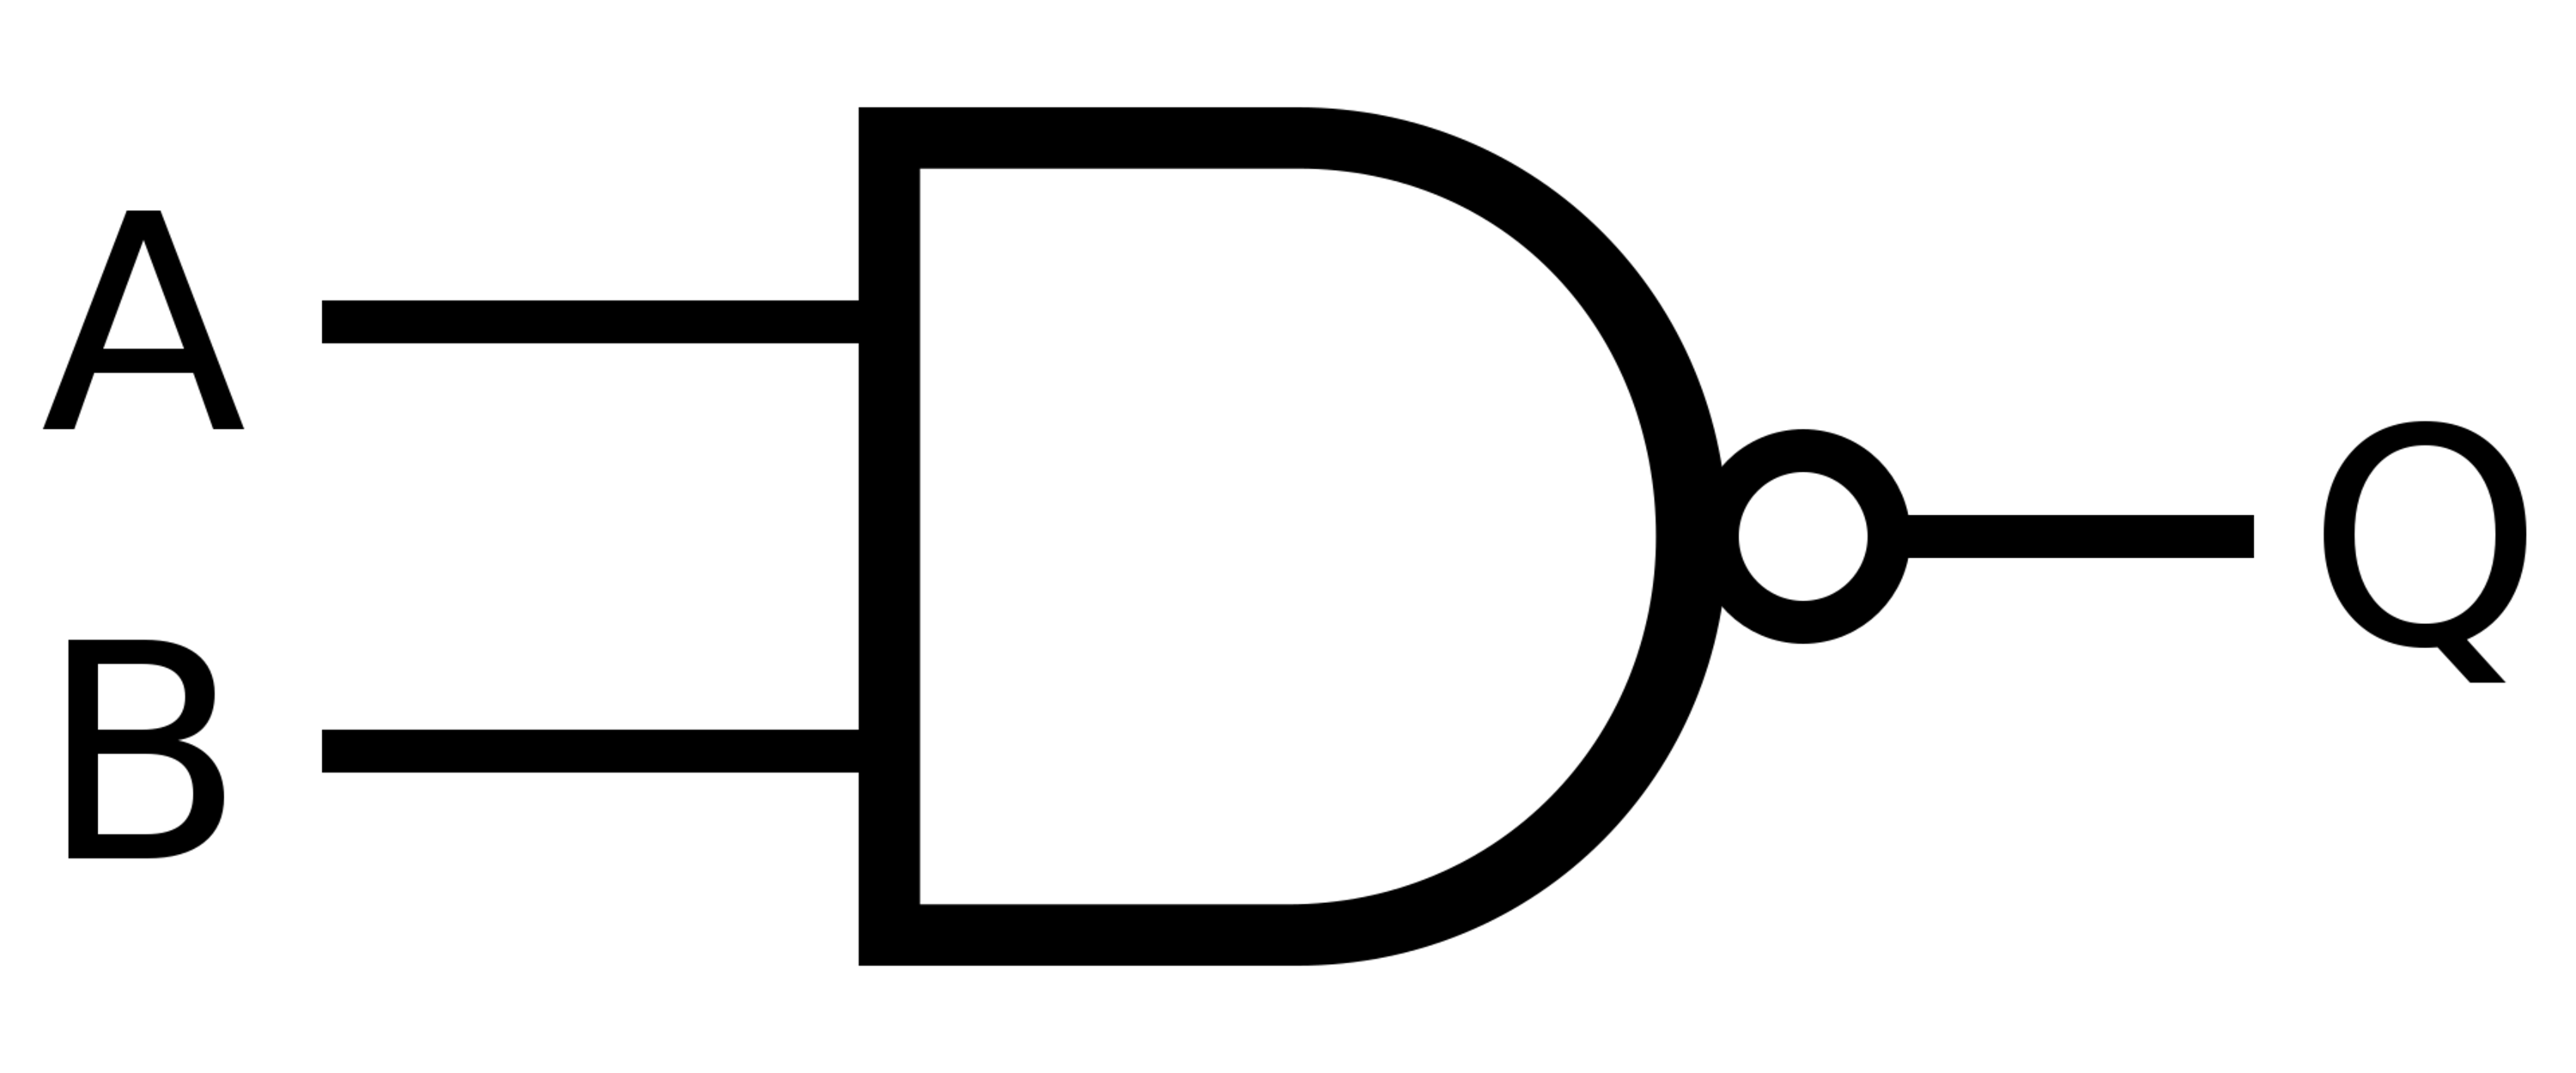
\includegraphics[width=3cm]{nand.pdf}
		\end{figure}
	
	\end{frame}		

	\subsection{Arquitetura de Von Neuman}

	\begin{frame}{\subsecname}
		\person{von-neuman.jpg}{John Von Neuman}{1903 - 1957}{3cm}{2cm}{2cm}
	\end{frame}
		
		
	\subsection{Lei de Moore}
	
	\comicfinal{moores-law.pdf}
	
	\begin{frame}{\subsecname}
		\person{moore.jpg}{Gordon Moore}{Intel, 1965}{3cm}{5cm}{3cm}
	\end{frame}

	\section{Computação Quântica}
	
	\subsection{Fenômenos Quânticos}
	
	\begin{frame}{\subsecname}
		\person{feynman.jpg}{Richard Feynman}{1918 - 1988}{3cm}{2cm}{2cm}
			
	\end{frame}
	
	\subsection{Postulados}
	
	\begin{frame}{\subsecname}
		\postulado{Representação}
		Um sistema físico isolado está associado a um espaço de Hilbert $\mathcal{H}$ e é, num dado momento no tempo, completamente descrito por um vetor unitário em $\mathcal{H}$, o estado do sistema.		
		\begin{align*}
			\ket{\Psi} \in \mathbb{C}^2 && (\mathbf{x} \in \mathbb{C}^2)\\
%%			\braket{\Psi}{\Psi} = 1 (\mathbf{x}^{\dagger} \mathbf{x} = 1)
		\end{align*}
		\vspace{-1cm} 
		\begin{figure}[H]
			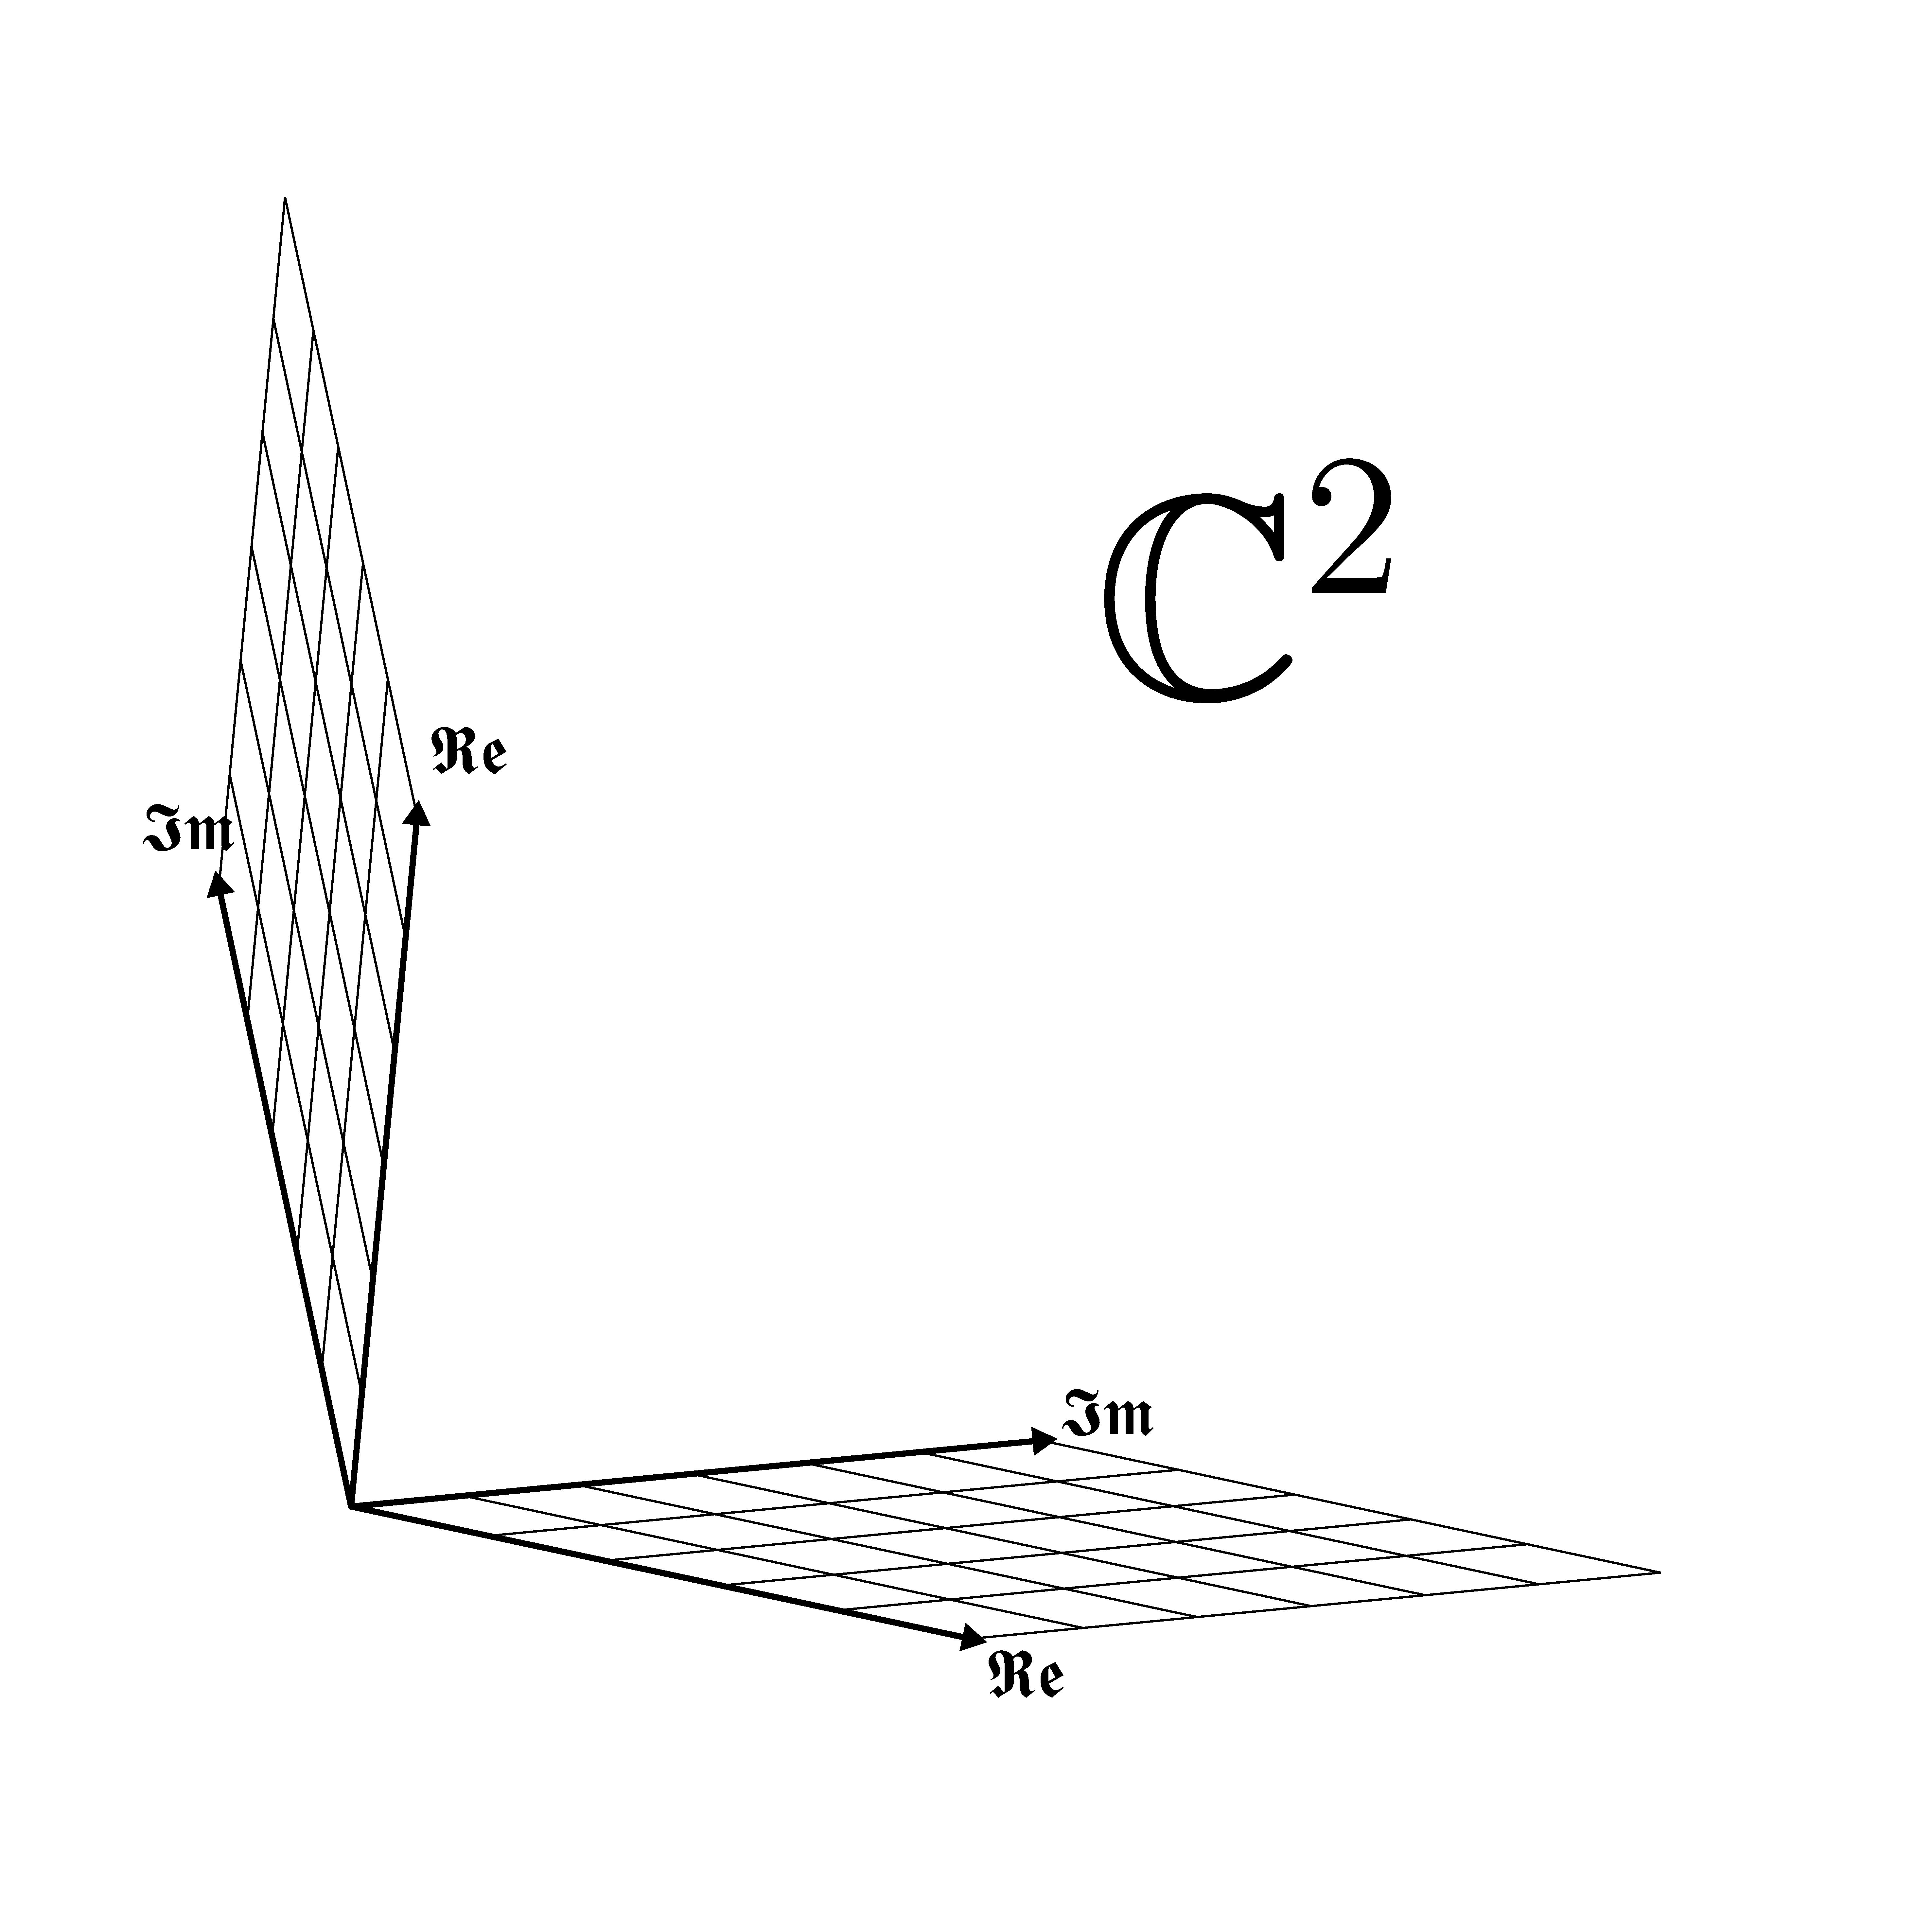
\includegraphics[width=5cm]{c2.pdf}
		\end{figure}
	\end{frame}
	
	\begin{frame}{\subsecname}
		\postulado{Representação}
		Um sistema físico isolado está associado a um espaço de Hilbert $\mathcal{H}$ e é, num dado momento no tempo, completamente descrito por um vetor unitário em $\mathcal{H}$, o estado do sistema.		
		\begin{align*}
			\ket{\Psi} \in \mathbb{C}^2 && (\mathbf{x} \in \mathbb{C}^2)\\
			\braket{\Psi}{\Psi} = 1 && (\mathbf{x}^{\dagger} \mathbf{x} = 1)
		\end{align*}
		\vspace{-1cm}
		\begin{figure}[H]
			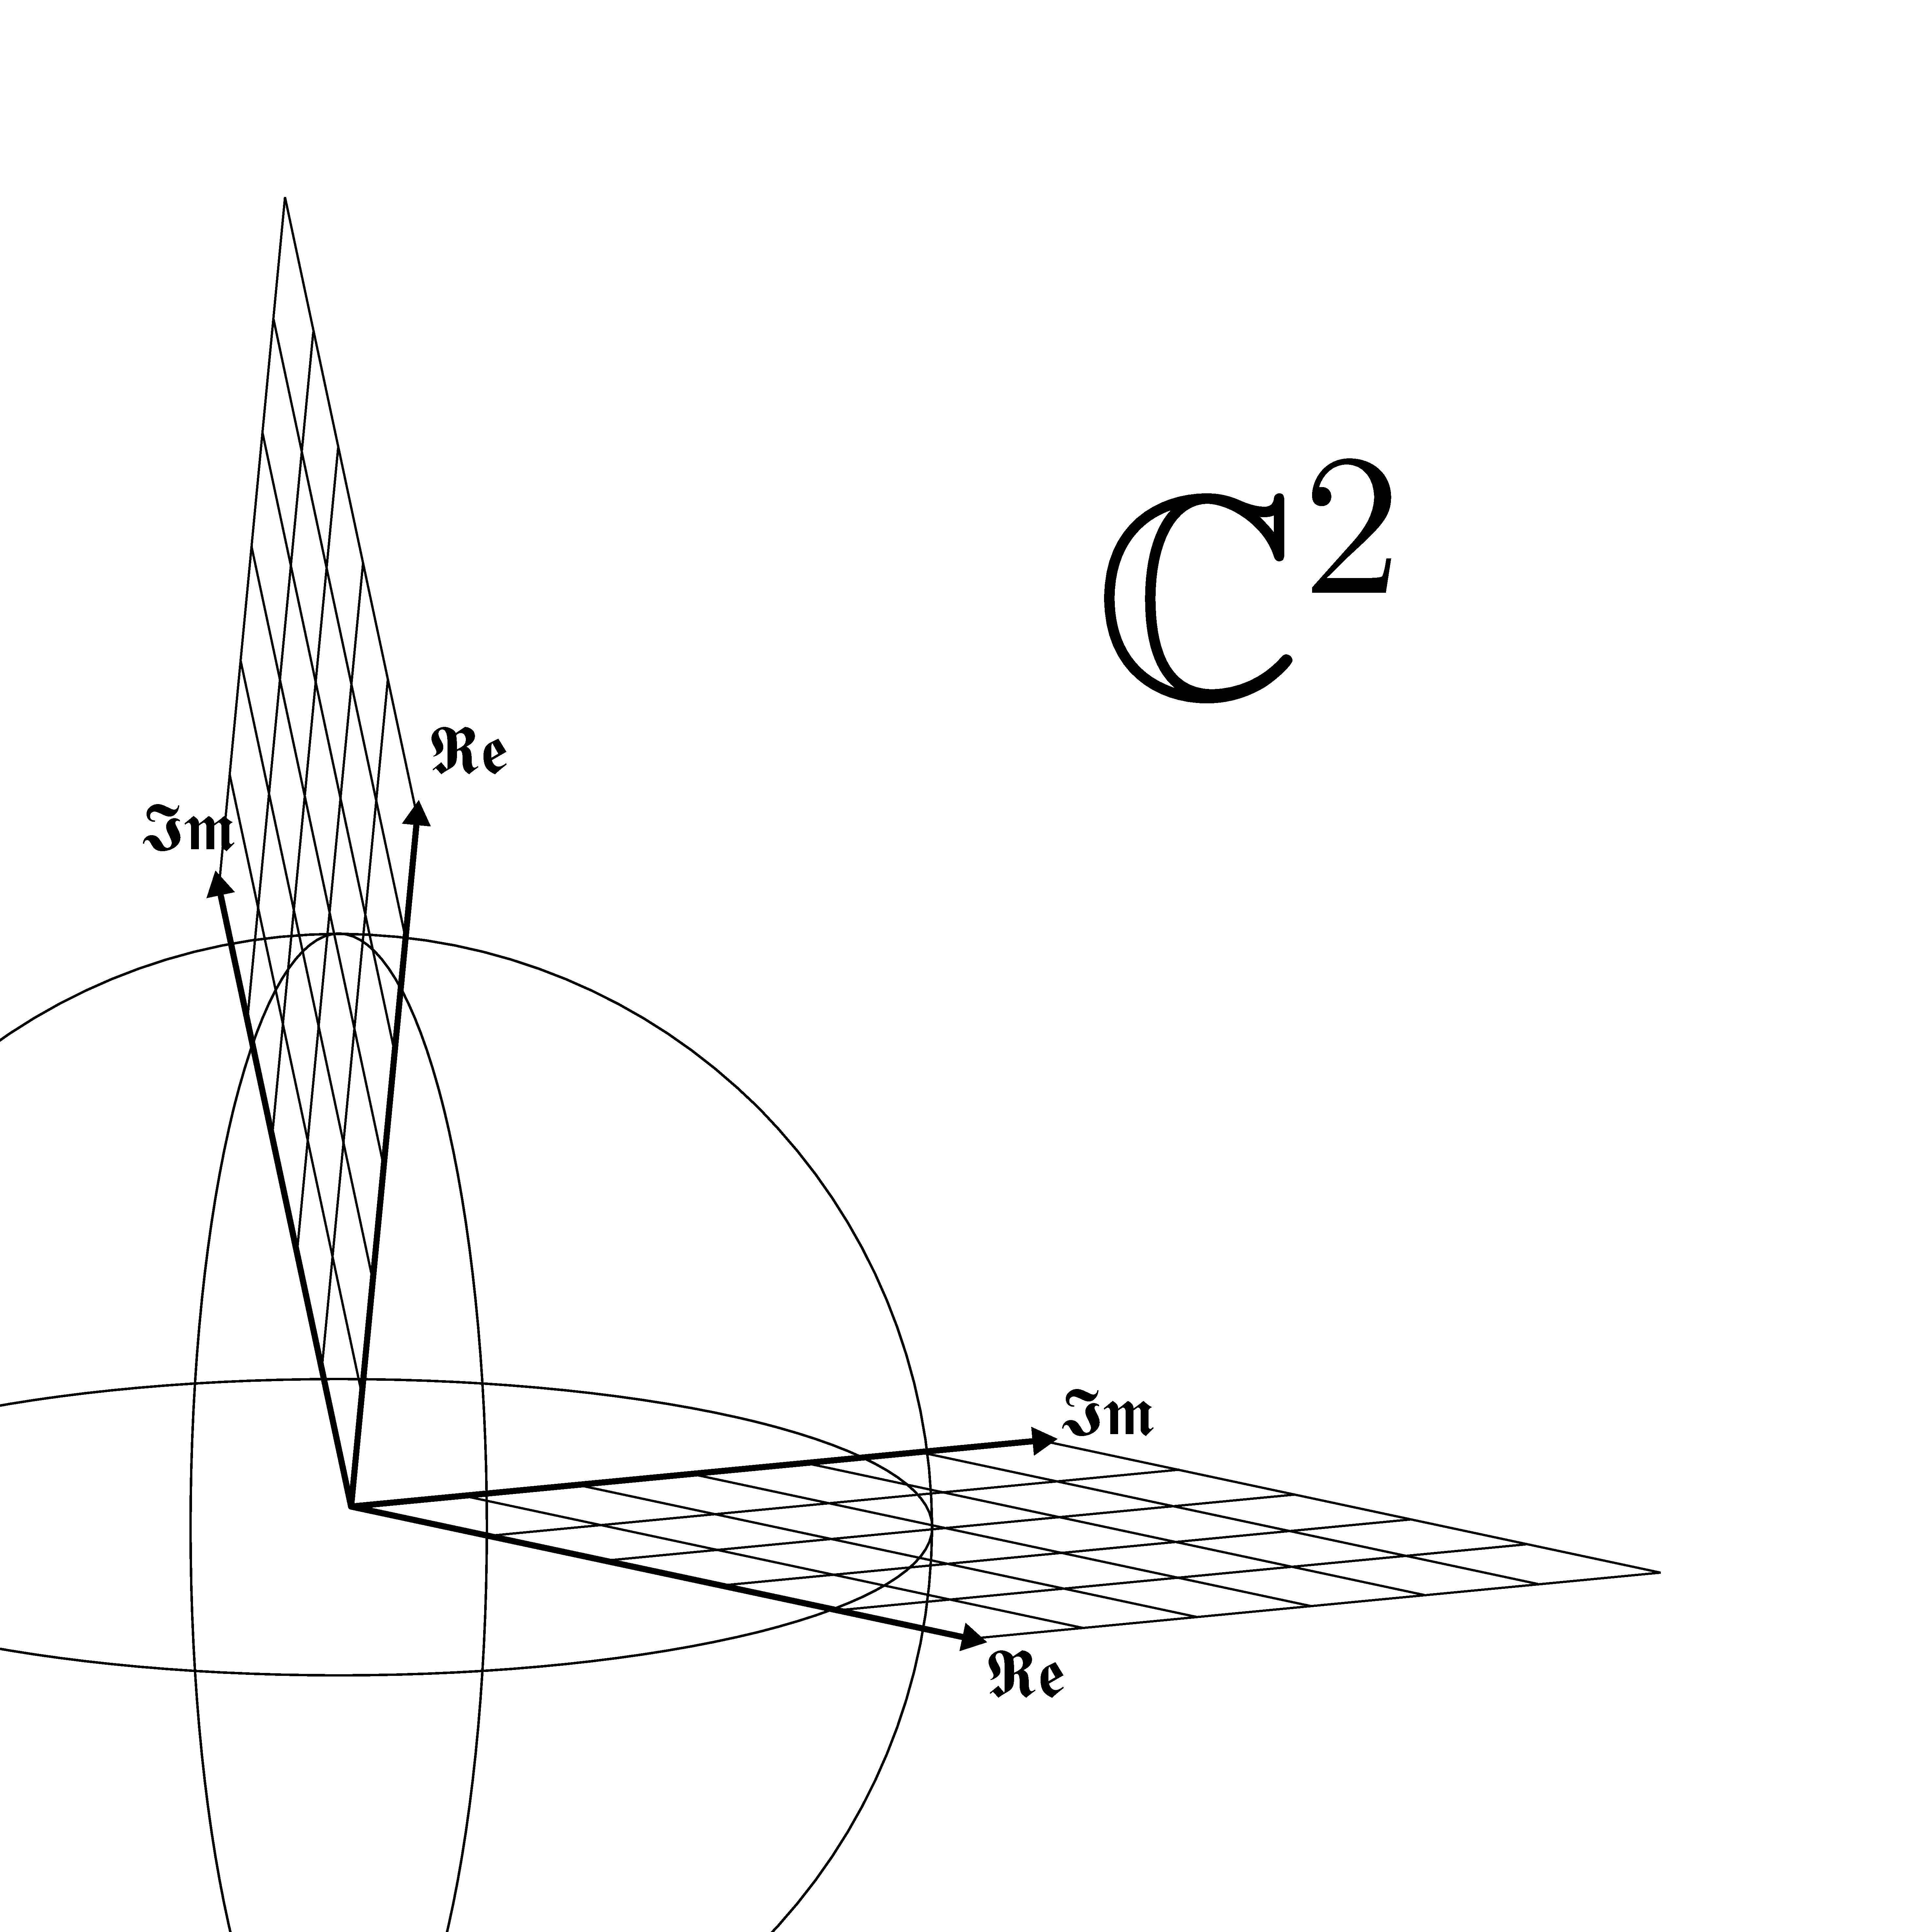
\includegraphics[width=5cm]{c2-sphere.pdf}
		\end{figure}
	\end{frame}

	\begin{frame}{\subsecname}
		\postulado{Composição}
		Um sistema é descrito pela composição dos estados que o representam, que se dá através do \emph{produto tensorial}.
		$$\ket{\Psi} \otimes \ket{\Phi} \equiv \ket{\Psi\Phi}$$
	\end{frame}
	
	\begin{frame}{\subsecname}
		\definicao{Produto de Kronecker}
		
		É um caso particular do \emph{produto tensorial}, computado da seguinte forma:
		
		\begin{align*}
		\mathbf{x} \otimes \mathbf{y} \equiv \vetor{x_1}{x_2} \otimes \vetor{y_1}{y_2} = \vetor{x_1 \vetor{y_1}{y_2} \vspace{2pt}}{x_2 \vetor{y_1}{y_2}} = \vetorx{x_1 y_1}{x_1 y_2}{x_2 y_1 }{x_2 y_2}
		\end{align*}
		
		Ele é bilinear e associativo, mas não é comutativo :(\\
	\end{frame}
	
	\begin{frame}{\subsecname}
		\definicao{Produto de Kronecker}
		
		Mas nem tudo está perdido. Tem outras propriedades legais também!\\
		
		Produto misto:
		\begin{align*}
			U \otimes V \cdot \ket{\Psi} \otimes \ket{\Phi} = U \ket{\Psi} \otimes V \ket{\Phi} && \mathbf{A} \otimes \mathbf{B} \cdot \mathbf{x} \otimes \mathbf{y} = \mathbf{A} \cdot \mathbf{B} \otimes \mathbf{x} \cdot \mathbf{y}
		\end{align*}
		
		Transposição:
		\begin{align*}
			(\ket{\Psi} \otimes \ket{\Phi})^\dagger &= \bra{\Psi} \otimes \bra{\Phi} && (\mathbf{x} \otimes \mathbf{y})^\dagger = \mathbf{x}^\dagger \otimes \mathbf{y}^\dagger\\
			\ket{\Psi\Phi}^\dagger &= \bra{\Phi\Psi} &&
		\end{align*}
		
		Existem outras, mas essas duas são as mais interessantes pra nós hoje.
	\end{frame}
	
	\begin{frame}{\subsecname}
		\definicao{Base Computacional}
		A \emph{Base Computacional} é determinada pelos estados ortogonais $\ket{0}$ e $\ket{1}$, definidos por
		\begin{align*}
		\ket{0} &= \vetor{1}{0}\\
		\ket{1} &= \vetor{0}{1}\\
		\end{align*}
		Chamaremos estes estados de \textit{qubits}!
	\end{frame}
	
	
	
	\begin{frame}{\subsecname}
		\definicao{Base Computacional}
		Construimos vetores de \textit{qubits} (registradores) através da composição:
		\footnotesize
		\begin{align*}
		\ket{00} = \ket{0} \otimes \ket{0} = \vetor{1}{0} \otimes \vetor{1}{0} = \vetorx{1}{0}{0}{0} &&
		\ket{01} = \ket{0} \otimes \ket{1} = \vetor{1}{0} \otimes \vetor{0}{1} = \vetorx{0}{1}{0}{0} \\
		~\\
		\ket{10} = \ket{1} \otimes \ket{0} = \vetor{0}{1} \otimes \vetor{1}{0} = \vetorx{0}{0}{1}{0} &&
		\ket{11} = \ket{1} \otimes \ket{1} = \vetor{0}{1} \otimes \vetor{0}{1} = \vetorx{0}{1}{0}{1}
		\end{align*}
		\normalsize
	\end{frame}
	
	\begin{frame}{\subsecname}
		\postulado{Evolução}
		A evolução de um sistema é descrita por um \textit{Hamiltoniano} $H$, representado por uma matriz Hermitiana, isto é, $H = H^{\dagger}$.\\
		
		Assim temos, pela equação de Schrödinger:
		$$H \ket{\Psi} =\ii \hslash \frac{d \ket{\Psi}}{dt} \implies \frac{d \ket{\Psi}}{dt} = \frac{-\ii}{\hslash} H \ket{\Psi}$$
		
		Sejam $\ket{\Psi(t_k)}$, $\ket{\Psi(t_{k+1})}$ os estados do sistema no tempo $t_k$ e $t_{k+1}$, respectivamente. Segue que:
		$$\ket{\Psi(t_{k+1})} = e^{\frac{-i H}{\hslash} (t_{k+1} - t_k)} \ket{\Psi(t_k)}$$
	\end{frame}
	
	\begin{frame}{\subsecname}
		\postulado{Evolução}
		\begin{enumerate}
			\item<1-> Seja $U = e^{\frac{-i H}{\hslash} (t_{k+1} - t_k)}$ o operador de evolução.
			\item<2-> Sabemos também que $U^{\dagger} = e^{\frac{i H^{\dagger}}{\hslash} (t_{k+1} - t_k)}$.
			\item<3-> Como a matriz $H$ é Hermitiana, temos que $U^{\dagger} U = I$.
		\end{enumerate}
		
	\uncover<4->{
	Podemos então dizer que a evolução dos sistemas se dá por operadores unitários!\\
	} \bigskip

	\vspace{1 cm}
	
	\uncover<5->{
	\centering\Huge
	Hora de conhecer alguns deles!
	}
	
	\end{frame}
	
	\begin{frame}{\subsecname}
		Matriz de Hadamard
		\begin{align*}
			H = \HH\\
		\end{align*}
	\end{frame}
	
	\begin{frame}{\subsecname}
		\begin{align*}
			H = \HH\\
			X = \XX\\
			Y = \YY\\
			Z = \ZZ
		\end{align*}
	\end{frame}
	
	\begin{frame}{Uma nota sobre reversibilidade}
		Para toda matriz unitária, como $U^{\dagger} U = U U^{\dagger} = I$, temos também que $U^\dagger = U^{-1}$.
	
		\textbf{O Princípio de Landau.}\\
		
		$$\Delta S > K T \log 2$$
		
	\end{frame}	
	
	\begin{frame}{\subsecname}
		\postulado{Medida}
	\end{frame}
	
	\subsection{Trapped-ion}
	\begin{frame}{\subsecname}
		Oi íon aprisionado
	\end{frame}

	\subsection{Algoritmos}
	
	\begin{frame}{Algoritmo de Grover}
	
	\person{grover.jpg}{Lov Grover}{Bell Labs}{3cm}{2cm}{2cm}
		
	\end{frame}

	\begin{frame}{Algoritmo de Shor}
	
	\person{shor.jpg}{Peter Shor}{MIT}{3cm}{2cm}{2cm}
			
	\end{frame}
	

	\subsection{Teletransporte Quântico}
	
	\comicw{quantum-teleportation.pdf}
	
	\begin{frame}{\subsecname}
	
		Imagine o teletransporte como um operador $\mathcal{T} : \ket{\Psi} \otimes \ket{\xi} \to \ket{\xi} \otimes \ket{\Psi}$
	
	\end{frame}
	
	\subsection{Teorema da não-clonagem}
	
	
	\begin{frame}{\subsecname}
	
	\teorema{Não-Clonagem}
		Não é possível fazer uma cópia de um estado quântico qualquer.

	\prova
	Vamos supor que existe um operador unitário $U$ capaz de clonar um estado $\ket{\Psi}$ qualquer, isto é:
		$$U (\ket{\Psi} \otimes \ket{\xi}) = \ket{\Psi} \otimes \ket{\Psi} = \ket{\Psi\Psi}$$
	Como isso vale para qualquer estado, também é preciso que
		$$U (\ket{\Phi} \otimes \ket{\xi}) = \ket{\Phi} \otimes \ket{\Phi} = \ket{\Phi\Phi}$$
	\end{frame}
	
	\begin{frame}{\subsecname}
		Tomando o produto interno entre $\ket{\Psi\Psi}$ e $\ket{\Phi\Phi}$:
		\begin{align*}
		\braket{\Psi\Psi}{\Phi\Phi} &= \bra{\xi\Psi}U^{\dagger} U \ket{\Phi\xi}\\
		&= \braket{\xi\Psi}{\Phi\xi}\\
		(\bra{\Psi} \otimes \bra{\Psi}) \cdot (\ket{\Phi} \otimes \ket{\Phi}) &= (\bra{\Psi} \otimes \bra{\xi}) \cdot (\ket{\Phi} \otimes \ket{\xi})\\
		\braket{\Psi}{\Phi} \otimes \braket{\Psi}{\Phi} &= \braket{\Psi}{\Phi} \otimes \braket{\xi}{\xi}\\
		\braket{\Psi}{\Phi}^2 &= \braket{\Psi}{\Phi}
		\end{align*}
		Portanto:
		\begin{align*}
			\braket{\Psi}{\Phi} = \begin{cases}
			1 \text{ se } \ket{\Psi} = \ket{\Phi}\\
			0 \text{ se } \ket{\Psi} \perp \ket{\Phi}\\
			\end{cases}\\
		&& \cqd
		\end{align*}
	\end{frame}
	
	\subsection{Fótons}	
	
	\begin{frame}{\subsecname}
		\imgw{superposition.pdf}{\textwidth}
	\end{frame}
	
	\subsection{Caminhadas Quânticas}
	
	\begin{frame}{\subsecname}
		\imgw{superposition.pdf}{\textwidth}
	\end{frame}

	\section{Computação Topológica}
	
	\subsection{Nós}
	
	\begin{frame}{\subsecname}
	
	\end{frame}	
	
	\begin{frame}{\subsecname}
	
	\end{frame}
	
	\subsection{Ânions}
	
	\begin{frame}{\subsecname}
	
	\end{frame}	
	
	\begin{frame}{\subsecname}
	
	\end{frame}
	
	\section{Computação Adiabática}
	
	\begin{frame}{\secname}
	\titulo{Equação de Pauli}
	$$\left[{\frac {1}{2m}}({\vec {\sigma }}\cdot ({\vec {p}}-q{\vec {A}}))^{2}+q\phi \right]\ket{\psi} = \ii\hbar {\frac {\partial }{\partial t}}\ket{\psi}$$
	
	\end{frame}
	
	\subsection{Teorema Adiabático}
	
	\subsection{Têmpera Quântica}	
	
	\begin{frame}{\subsecname}
		\begin{align*}
			H(t) = &-\frac{A(t)}{2}  \sum_{i} h_i \cdot X\ket{s_i}\\ &+ \frac{B(t)}{2}\left(\sum_{i} h_i \cdot Z\ket{s_i} + \sum_{i < j} J_{i,j} \cdot Z\ket{s_i} \otimes Z\ket{s_j}\right)
		\end{align*}
	\end{frame}
	
	\begin{frame}{\subsecname}
		\imgw{energy-levels.pdf}{9cm}
	\end{frame}
	
	\section{Fim?}
	
	\subsection{Saltos Quânticos}
	
	\begin{frame}{\subsecname}
		\imgh{enclave-map.pdf}{\textheight}
	\end{frame}

	\begin{frame}{\subsecname}
		\imgw{enclave-chart.pdf}{\textwidth}
	\end{frame}

	\subsection{Supremacia Quântica}
	
	\comicw{quantum.pdf}
	
	\comicw{failure.pdf}
	
	\begin{frame}{\subsecname}
		\person{kalai.jpg}{Gil Kalai}{Yale \& Huji}{4cm}{2cm}{2cm}
	\end{frame}	
	
	\begin{frame}{\subsecname}
		\textbf{Definição um tanto vaga. (Supremacia Quântica)}\\
		Atingir a supremacia quântica significa realizar uma tarefa em um computador quântico que não se possa concretizar no clássico.
	\end{frame}	
	
	\begin{frame}{\subsecname}
	
	\end{frame}
	
	\subsection{Material}
	
	\begin{frame}{\subsecname}
		\begin{itemize}
			\item The Quantum Algorithm Zoo
			\item Quanta Magazine
		\end{itemize}
	
	\end{frame}
	
	\begin{frame}
		Obrigado
	\end{frame}
	
	\subsection{Bibliografia}
	
	\begin{frame}{\subsecname}
		\thebibliography{99}
		
		\bibitem{field:2018} \textbf{Introduction to topological quantum computation with non-Abelian anyons}, FIELD, B. \& SIMULA, T., School of Physics and Astronomy, Monash University, Victoria 3800, Australia.
		
		\bibitem{}
	\end{frame}
	
	\section*{Reprograme o seu DNA na frequência do Sucesso}
	
	\begin{frame}
	
	\end{frame}
\end{document}